\documentclass{beamer}
\usepackage{feynmp}
\DeclareGraphicsRule{*}{mps}{*}{}
\usepackage{beamerthemesplit}
\usepackage{slashed}
\usepackage{cancel}
\usetheme{Boadilla}
\usecolortheme{seahorse}
%% \definecolor{meerkat-blue}{HTML}{0090CA}

%% \setbeamercolor*{titlelike}{bg=meerkat-blue,fg=black}
%%  \setbeamercolor*{title page}{bg=meerkat-blue,fg=black}
%%  \setbeamercolor*{block title}{bg=meerkat-blue}
%%  \setbeamercolor*{palette secondary}{use=structure,fg=white,bg=meerkat-blue}
%%  \setbeamercolor*{palette tertiary}{use=structure,fg=white,bg=meerkat-blue}
%%  \setbeamercolor*{palette quaternary}{use=structure,fg=white,bg=meerkat-blue}

 \setbeamertemplate{navigation symbols}{}%remove navigation symbols
\title[Public Health Surveillance]{Technical introduction to Public Health Surveillance System}
\author{Gunnar, Jonathan, Mix and Jyri (WHO development team)}
\institute[WHO]{World Health Organisation}
\date{\today}



\begin{document}

\begin{frame}
\titlepage
\end{frame}

\begin{frame}
\tableofcontents
\end{frame}

\section{Overview and Introduction}
%% 20 min
\begin{frame}
  \frametitle{Plan}

  \textbf{Tuesday:}\\
  	1. Introduction \\
	2. Setup: Linux, Docker, git \\
	3. Introduction to Python\\
  \textbf{ Wednesday:}\\
	4. Web Programming in Python \\
	5. Preparing tablet forms \\
	6. Databases (with Python) \\
  \textbf{Thursday:}\\
  	7. JavaScript\\
	8. Using Meerkat Demo system\\
  \textbf{ Friday:}\\
  	9. Using Meerkat Demo system\\
  
\end{frame}
\begin{frame}
  \frametitle{Mission statement}

  \begin{block}{Public health surveillance mission statement}
    To enable real-time case-based surveillance at the health facility level that improves public health and clinical decision making at all levels of the health system.
  \end{block}
  \vspace{10pt}
  To this end the we want to develop secure and reliable technical solutions that fulfil the following principles:

  
  \begin{itemize}
  \item Configurable services
  \item A micro-service architecture
  \item Supporting multiple data source and multiple data outputs
    \item Open source
  \end{itemize}
\end{frame}  

\begin{frame}
  \frametitle{Current Status}

  \begin{itemize}
  \item 15 districts
  \item 385 facilities
  \item  39 733 submitted case reports
  \item 162 077 consultations
  \end{itemize}
\end{frame}


\section{Principles of implementation}

\begin{frame}
  \frametitle{Microservices Architecture}
  We aim to design the system so that we have a system of loosely coupled smaller services performing a self contained range of functions.

  \begin{itemize}
  \item Each component has a clearly defined limited scope
  \item Each component should be independently deployable
  \item Components are mainly coupled through APIs
  \item Made much easier by Docker
  \end{itemize}

  Benefits:

  \begin{itemize}
  \item Each component can be developed independently
  \item Can make different design decisions for each component
  \item Components can be easily replaced if needed
  \item Separation of responsibilities and non repetition of code
    \end{itemize}
\end{frame}

\begin{frame}
  \frametitle{Open Source}
  We only use open source components and release all code as open source.

  \vspace{30pt}
  
  Using open source brings many benefits:

  \begin{itemize}
  \item No licensing costs etc. 
  \item Other groups can use and improve our software
  \item Can determine in detail how everything works if needed
  \item Much industry leading software is open source
  \end{itemize}

\end{frame}
\begin{frame}
  \frametitle{Continuous Integration}
  We develop our software on a continuous release cycle that can always be deployed.\\
  \vspace{5pt}
  Made possible by:
  \begin{itemize}
  \item Version control via git
  \item Unit-testing and automatic testing on code push (Travis)
  \item Nightly builds of development branch
  \item Automatic build and deploy process
  \item Flexible infrastructure in the cloud
  \end{itemize}
  \vspace{5pt}
  Benefits:
  \begin{itemize}
  \item Faster deployment of needed changes
  \item Continuous feedback on changes and incremental improvements
  \end{itemize}

\end{frame}




\section{Technical Structure}
%% 30 min
\begin{frame}
  \frametitle{Current Data Flow}
  \begin{center}
    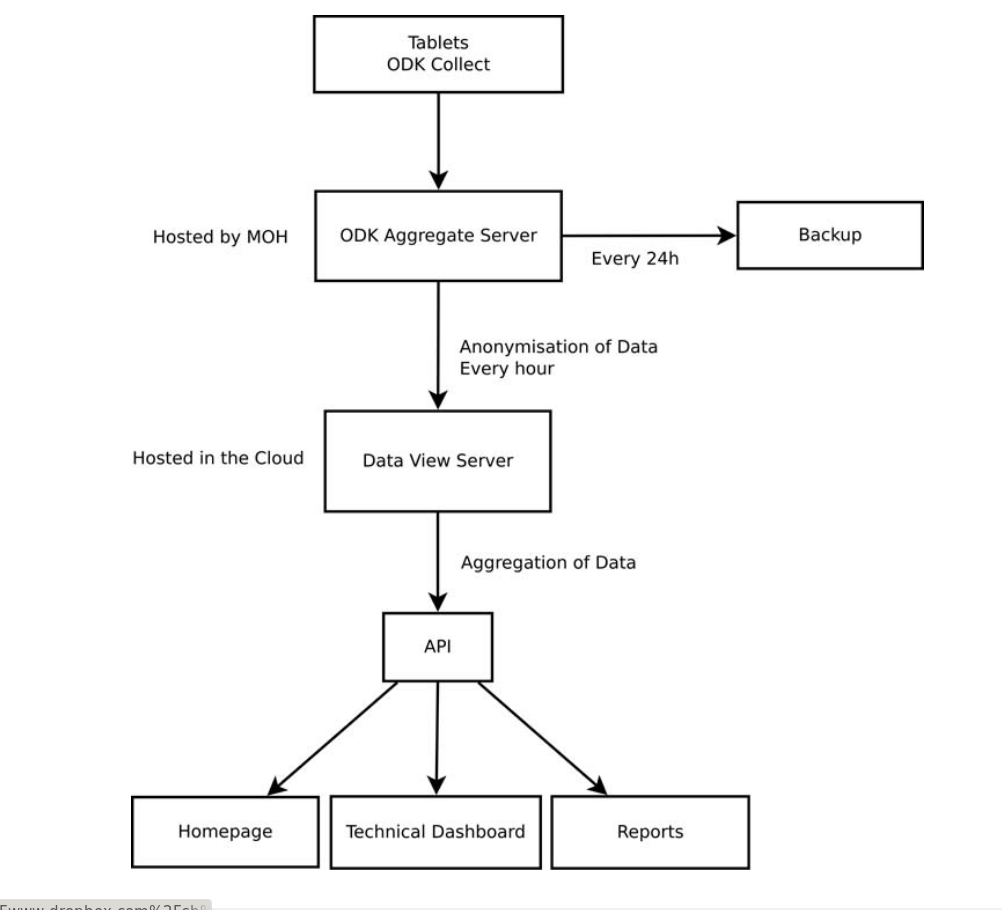
\includegraphics[width=9cm]{data_flow.png}
  \end{center}
\end{frame}

\begin{frame}
  \frametitle{Data Flow}
  The main function of the software is to get the information from the tablets to the users in a useful format. \\
  \vspace{10pt}

  We want to support many different sources of data and different formats. \\

    \vspace{10pt}
  
  E.g: Gender might be coded as M/F in variable gen in one form and as male/female in variable pt1./gender in another. \\

    \vspace{10pt}
  
    To overcome this we process all the raw data using configurable codes so that both way of specifying gender can be combined. The end point of this is a clean data table which can easily be used for aggregation. \\

    \vspace{10pt}
    This data can then be used to power the websites and other data displays

    
  \end{frame}


\subsection{Data Collection}

\begin{frame}
  \frametitle{Data Collection}
  Data collection modalities:
  \begin{itemize}
  \item Forms submitted from tablets (Main modality)
  \item Automatic status messages from tablets (Under development)
  \item Uploading spreadsheets (Experimental feature)
  \item Data from other sources via APIs (Future)
  \end{itemize}

  \vspace{10pt}
  All collected data will be stored on the servers in the Ministry and is owned by the Ministry. 
\end{frame}


\begin{frame}
  \frametitle{Data collection from tablets}
  \begin{itemize}
  \item Android tablets that run custom version of ODK Collect
  \item Automatic synchronisation of app and forms
  \item Automated configuration
  \item Forms are created in Excel (XLS forms)
  \item http://xlsform.org/
  \item Automatic status messages via Google Cloud Messaging
  \item Tablet management needs to be improved
  \end{itemize}
\end{frame}
\begin{frame}
  \frametitle{Data Collection Server}
  \begin{itemize}
  \item Server in the Ministry Data Centre (to be moved here next week)
  \item Ubuntu Linux operating system
  \item Full disk encryption and modern security
  \item Runs ODK Aggregate software
  \item Java application running in Tomcat behind Nginx
  \item Custom built daily backup
  \item Anonymised export of data to AWS cloud
  \end{itemize}
\end{frame}

\subsection{Data processing}
\begin{frame}
  \frametitle{Data Processing}
  This service starts with the raw anonymised data and provides aggregated data for display
  \begin{itemize}
  \item Configurable codes are used to translate raw data into useful data
  \item These codes provide a flexible way of giving meaning to the data.
  \item Support: Matching, calculated values, number in interval, multiple conditions etc
  \item Data processing tools also deal with important meta data like locations and tablets.
  \item Data is localised by matching on device-ids
  \item Provide an API that gives access to data
  \item Supports a wide range of aggregated data views.
  \item Data processing has two components Abacus and API
  \end{itemize}
\end{frame}



\begin{frame}
  \frametitle{Meerkat Abacus}
  \begin{itemize}
  \item Python package that imports raw data and meta data and processes the data to the finished data table
  \item Scheduled updates every hour using Celery
  \item Uses a PostgreSQL database and SqlAlchemy (see tomorrow)
  \item When processing data alerts are identified and sent out
  \item Supports both single and threshold alerts
  \item Supports codes based on linking multiple form entries
  \item Data sources, locations, codes and links configurable
  \item https://github.com/meerkat-code/meerkat\_abacus
  \end{itemize}

\end{frame}

\begin{frame}
   \frametitle{Example}
  \begin{center}
    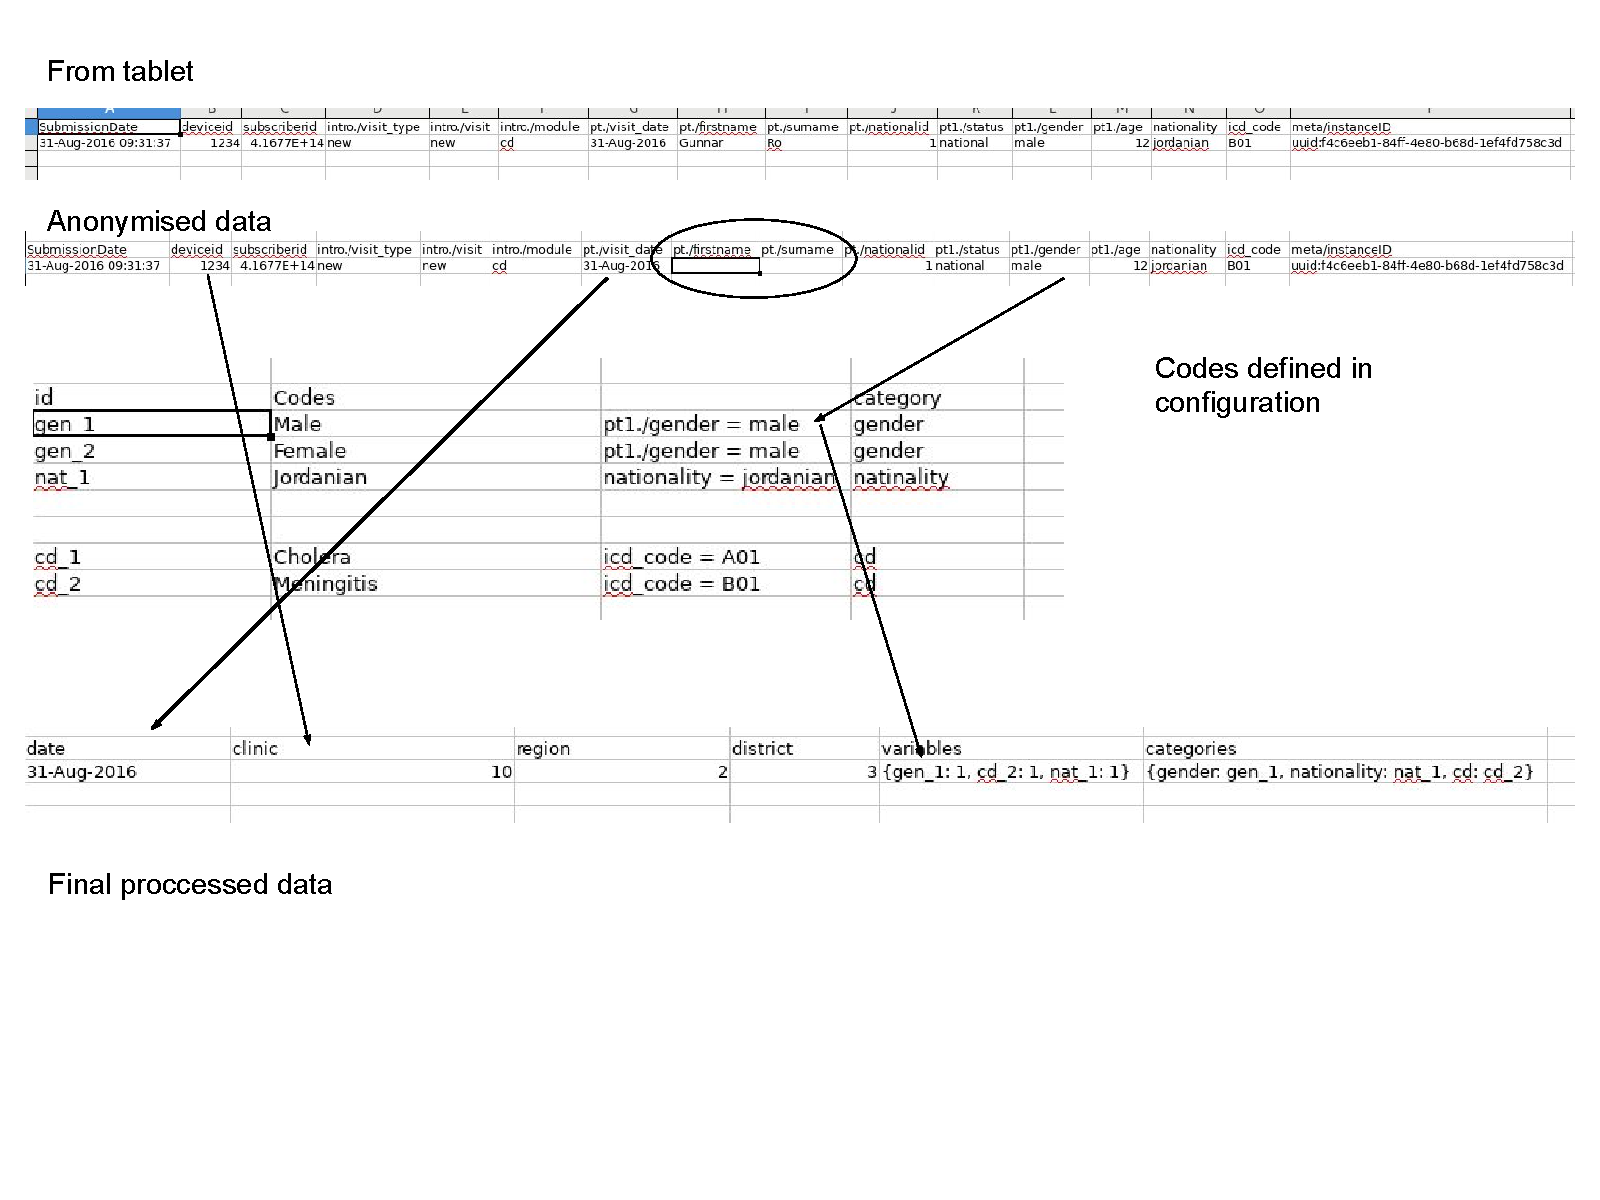
\includegraphics[width=11cm]{ex.pdf}
  \end{center}

\end{frame}



\begin{frame}
    \frametitle{Meerkat Api}
    \begin{itemize}
    \item Python package that provides an HTTP rest API to query data
    \item Based on Flask (see tomorrow)
    \item Used Pandas for some of the data aggregations
    \item Supports aggregation over time and location
    \item Mapping of cases, incidence rates and clinics
    \item Supports many reports
    \item Supports explore data functionality
    \item Supports downloading the raw data using a Celery as task runner
    \item For the API only the processed data is used
    \item https://github.com/meerkat-code/meerkat\_api
    \end{itemize}
\end{frame}

\subsection{Web interface}
\begin{frame}
  \frametitle{Meerkat Frontend}
  \begin{itemize}
  \item Written in Python and HTML, JS, CSS
  \item Uses many open source libraries. E.g bootstrap and Highcharts
  \item Includes public homepage and then a private technical page
  \item Technical page includes data on demographics, morbidity, completeness, PIP and alerts
  \item Very configurable, can change the number and content of the tabs
  \item The technical site also includes download data, explore data and reports
  \item https://github.com/meerkat-code/meerkat\_frontend
  \item {\bf Meerkat Hermes}: Separate microservice to sends email and SMS notifications and administer notifications
  \end{itemize}
\end{frame}
\begin{frame}
  \frametitle{Authentication}
  \begin{itemize}
  \item The frontend supports many different user accounts and access levels
  \item Each component and each tab can have different access levels. 
  \item Authentication is implemented as a separate microservice
  \item Written in Python and HTML, JS, CSS
  \item Uses encrypted JSON webtokens to communicate access rules
  \item We have user accounts and roles
  \item Completely flexible access role network
  \item https://github.com/meerkat-code/meerkat\_authentication
  \end{itemize}
\end{frame}



\begin{frame}
  \frametitle{Software review}
  \begin{itemize}
  \item Operating system: Linux (mainly ubuntu) (Today)
  \item Containerisation: Docker and AWS ECS (Today)
  \item Python (Today), Flask, Celery, SqlAlchemy (Tomorrow)
  \item JS (gulp, highcharts, bootstrap, jquery), HTML, CSS (Thursday)
  \item Databases: PostgreSQL (tomorrow) and DynamoDB 
  \item Version control: git (Today)
  \end{itemize}
\end{frame}

\begin{frame}
  \frametitle{Important programming libraries}
  {\bf Python:} \\
  flask : micro-framework for web programming \\
  SqlAlchemy: Database abstraction \\
  pandas: Data analysis \\
  shapely: GIS \\

  \vspace{10pt}

  {\bf Javascript:} \\
  jQuery: DOM manipulation \\
  bower: asset management \\
  gulp: task runner \\
  
\end{frame}

\subsection{Infrastructure}
\begin{frame}
  \frametitle{Meerkat Infrastructure}
  \begin{itemize}
  \item Use docker for containerisation for both production and development
  \item A github repository for every country and a demo country
  \item Data collection server is physical server in the Ministry
  \item Website and all other resources in AWS cloud
  \item Each country has separate infrastructure in the cloud
  \item We use Travis for automatic testing
  \item Have nightly builds of ``development'' servers
  \end{itemize}
\end{frame}

\begin{frame}
  \frametitle{AWS Infrastructure}
  \begin{itemize}
  \item S3 for storage: Anonymised data, encrypted backups, forms and packages for tablets
  \item Route53, VPC for dns and internal networking. All of our servers live in a private virtual network.
  \item EC2 for virtual servers. This gives create flexibility in terms of number and size of servers
  \item ECS for orchestrating docker. For managing servers, repositories and task definitions
  \item OpsWorks for server management. Using Chef
  \item DynamoDB(noSQL) and hosted version of PostgreSQL 
  \item SES: For sending emails
  \end{itemize}
\end{frame}


\begin{frame}
  \frametitle{Questions}
  \Huge Questions?
\end{frame}

\end{document} 
